\documentclass[10pt,a4paper]{article}

% -------------------------------------------------
% Encodage et langue
% -------------------------------------------------
\usepackage[utf8]{inputenc}
\usepackage[T1]{fontenc}
\usepackage[french]{babel}
\usepackage{lmodern}

% -------------------------------------------------
% Mise en page
% -------------------------------------------------
\usepackage{geometry}
\geometry{margin=0.95cm,top=0.85cm,bottom=0.95cm}

% -------------------------------------------------
% Packages graphiques et tableaux
% -------------------------------------------------
\usepackage{graphicx}
\usepackage[table]{xcolor}
\usepackage{tabularx}
\usepackage{array}
\usepackage{booktabs}
\usepackage{multicol}
\usepackage{tcolorbox}
\usepackage{enumitem}
\usepackage{hyperref}
\usepackage{ragged2e}

% -------------------------------------------------
% Couleurs
% -------------------------------------------------
\definecolor{bleuPCB}{HTML}{0B3A7A}
\definecolor{vertPCB}{HTML}{0B7F55}
\definecolor{orangePCB}{HTML}{F59E0B}
\definecolor{rougePCB}{HTML}{DC2626}

% -------------------------------------------------
% Reglages generaux
% -------------------------------------------------
\setlength{\parindent}{0pt}
\setlength{\parskip}{2pt}

\setlist[itemize]{nosep,leftmargin=1.1em}
\setlist[enumerate]{nosep,leftmargin=1.2em}

\renewcommand{\arraystretch}{1.12}

\newcolumntype{Y}{>{\RaggedRight\arraybackslash}X}
\newcolumntype{L}[1]{>{\RaggedRight\arraybackslash}p{#1}}

\pagestyle{empty}

% -------------------------------------------------
% Debut document
% -------------------------------------------------
\begin{document}

\begin{center}
{\LARGE\bfseries\color{bleuPCB} EmbedLab Board -- Fiche de prise en main rapide}
\hfill
{\bfseries V1.0}\\
{Carte pedagogique pour GPIO, ADC, UART, I2C, affichage, capteurs et actionneurs}
\end{center}

\vspace{-0.1cm}

\begin{minipage}{0.62\textwidth}
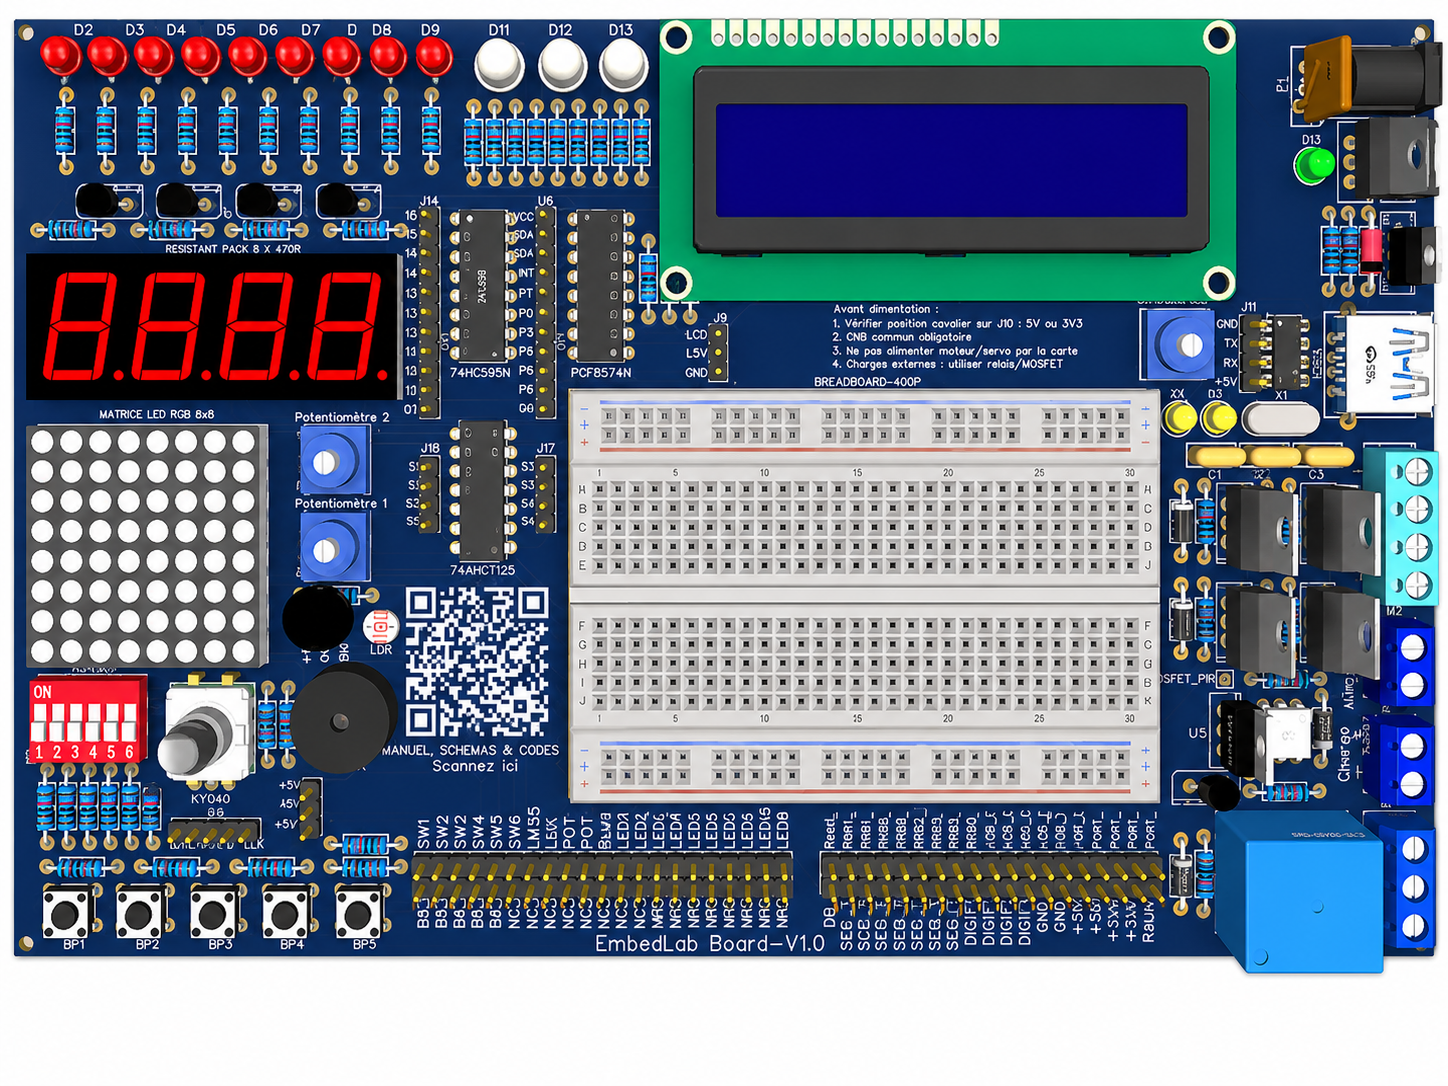
\includegraphics[width=\textwidth]{../figures/cover_photo.png}
\end{minipage}
\hfill
\begin{minipage}{0.35\textwidth}

\begin{tcolorbox}[
colback=orangePCB!10,
colframe=orangePCB,
title=Avant alimentation,
fonttitle=\bfseries
]
\begin{enumerate}
\item Verifier \textbf{J10 : 5 V ou 3,3 V}.
\item Relier le \textbf{GND} de la carte au \textbf{GND} du microcontroleur.
\item Ne pas alimenter moteur ou servo depuis le 7805.
\item Charges externes : utiliser \textbf{relais}, \textbf{MOSFET} ou \textbf{pont en H}.
\item Couper l'alimentation avant toute modification de cablage.
\end{enumerate}
\end{tcolorbox}

\begin{tcolorbox}[
colback=rougePCB!7,
colframe=rougePCB,
title=J10 est critique,
fonttitle=\bfseries
]
5 V : Arduino Uno/Nano/MEGA.\\
3,3 V : ESP32, STM32, FPGA, Pico.\\
Verifier J10 avant POT1, POT2, LM35, LDR et toute entree ADC.
\end{tcolorbox}

\end{minipage}

\vspace{0.12cm}

{\small
\begin{tabularx}{\textwidth}{@{}L{0.7cm}L{3.0cm}Y L{0.7cm}L{3.0cm}Y@{}}
\toprule
\rowcolor{bleuPCB!12}
\textbf{N} & \textbf{Zone} & \textbf{Role} &
\textbf{N} & \textbf{Zone} & \textbf{Role} \\
\midrule
1 & LEDs rouges & sorties logiques simples &
12 & SN74AHCT125 & adaptation 3,3 V vers 5 V \\

2 & LEDs RGB & PWM / couleurs &
13 & QR code & acces documentation et fichiers \\

3 & LCD 1602 & messages et mesures &
14 & Breadboard 400 pts & prototypage rapide \\

4 & Alimentation & 12 V, PTC, 5 V, 3,3 V &
15 & Pont en H & petit moteur DC \\

5 & 7 segments 4 digits & affichage multiplexe &
16 & MOSFET & charge DC externe \\

6 & 74HC595N & extension de sorties &
17 & DIP-switch & configuration \\

7 & PCF8574N & extension I2C &
18 & KY040 & encodeur rotatif \\

8 & Zone rappel / J9 & consignes rapides &
19 & Buzzer & alarme sonore \\

9 & CH340G / USB & UART PC &
20 & BP1 a BP5 & boutons poussoirs \\

10 & Matrice 8x8 & animation / balayage &
21 & Headers & acces aux signaux \\

11 & POT, LM35, LDR & entrees analogiques &
22 & Relais & charge basse tension \\
\bottomrule
\end{tabularx}
}

\vspace{0.15cm}

\begin{multicols}{2}

\section*{Connecteurs rapides}

{\small
\begin{tabularx}{\linewidth}{@{}L{1.8cm}Y@{}}
\toprule
\rowcolor{bleuPCB!12}
\textbf{Repere} & \textbf{Usage} \\
\midrule
J1 & LEDs rouges D1 a D10 \\
J2 & LEDs RGB D11 a D13 \\
J3 & Buzzer \\
J4 & BP1 a BP5 \\
J5 & Commande MOSFET \\
J6 & Commande pont en H \\
J7 / J8 & Commande Matrice 8x8 \\
J9 & Entrees analogiques LM35, LDR, POT1, POT2 \\
J10 & Selection 5 V / 3,3 V \\
J11 & USB-serie : GND, TX, RX, +5 V \\
J12 & Encodeur KY040 \\
J13 & Sorties Q0 a Q7 du 74HC595N \\
J14 & Commande 74HC595N : DS, ST, SH \\
J15 & E/S P0 a P7 du PCF8574N \\
J16 & Bus PCF8574N : SDA, SCL, INT \\
J17 / J18 & SN74AHCT125 \\
J19 & Alimentation LCD \\
H1 & Pilotage de l'afficheur 7 segments 4 digits \\
P6 & Pilotage de l'ecran LCD \\
P8 & Sorties disponibles pour alimenter le breadboard \\
10K1 &  Commande la charge AC/DC apartir du relais \\

\bottomrule
\end{tabularx}
}

\section*{Procedure rapide}

\begin{enumerate}
\item Choisir un module a tester.
\item Regler J10 selon la carte externe.
\item Relier le GND commun.
\item Cabler le signal vers le header correspondant.
\item Alimenter puis televerser un code minimal.
\item Mesurer si le resultat n'est pas conforme.
\end{enumerate}

\section*{Limites conseillees en TP}

\begin{itemize}
\item Entree carte : 12 V DC stable, polarite respectee.
\item 5 V logique : ne pas tirer de forte puissance sur le LM7805.
\item Relais : charge DC basse tension uniquement.
\item MOSFET : charge DC externe, alimentation separee si besoin.
\item Pont en H : petit moteur DC basse tension.
\item USB : debug et UART, pas pour moteurs.
\end{itemize}

\end{multicols}

\newpage

\begin{center}
{\Large\bfseries\color{bleuPCB} EmbedLab Board -- raccordements essentiels}\\
{Page 2 : analogique, communication, puissance et depannage}
\end{center}

\begin{multicols}{2}

\section*{Raccordement analogique}

\begin{tcolorbox}[
colback=orangePCB!10,
colframe=orangePCB,
title=Regle ADC,
fonttitle=\bfseries
]
Le signal analogique ne doit jamais depasser la tension acceptee par le microcontroleur. Verifier donc la position de \textbf{J10} avant d'utiliser POT1, POT2, LM35 ou LDR.
\end{tcolorbox}

{\small
\begin{tabularx}{\linewidth}{@{}L{2.1cm}Y@{}}
\toprule
\rowcolor{bleuPCB!12}
\textbf{Carte externe} & \textbf{Position de J10} \\
\midrule
Arduino 5 V & J10 sur 5 V \\
ESP32 / STM32 & J10 sur 3,3 V \\
FPGA / Pico & J10 sur 3,3 V \\
Mesure & Verifier au multimetre avant connexion \\
\bottomrule
\end{tabularx}
}

\section*{USB-serie}

{\small
\begin{tabularx}{\linewidth}{@{}L{2.2cm}Y@{}}
\toprule
\rowcolor{bleuPCB!12}
\textbf{Element} & \textbf{Usage} \\
\midrule
J11 & GND, TX, RX, +5 V \\
LEDs TX/RX & Visualisation de l'activite UART \\
Usage & Terminal serie, debug, donnees capteurs \\
Precaution & Croiser TX carte vers RX microcontroleur \\
\bottomrule
\end{tabularx}
}

\section*{Puissance basse tension}

{\small
\begin{tabularx}{\linewidth}{@{}L{2.1cm}Y@{}}
\toprule
\rowcolor{bleuPCB!12}
\textbf{Bloc} & \textbf{Recommandation} \\
\midrule
Relais & Charge DC basse tension, pas de secteur 230 V en TP \\
MOSFET & Charge DC externe, commande par J5 \\
Pont en H & Petit moteur DC, commandes dediees \\
Alim moteur & Alimentation externe recommandee \\
Masse & GND commun sauf montage isole \\
\bottomrule
\end{tabularx}
}

\section*{Depannage express}

{\small
\begin{tabularx}{\linewidth}{@{}L{2.1cm}Y@{}}
\toprule
\rowcolor{bleuPCB!12}
\textbf{Symptome} & \textbf{Action} \\
\midrule
Aucune alim & verifier 12 V, polarite, PTC, court-circuit \\
ADC faux & verifier J10 et GND commun \\
LCD vide & verifier J9/J19, contraste, cablage \\
USB absent & pilote CH340, cable, port COM \\
Moteur KO & verifier alimentation externe et commandes pont en H \\
Chauffe & debrancher charges, ne pas tirer sur le 7805 \\
\bottomrule
\end{tabularx}
}

\section*{QR code du depot}

\begin{center}

\includegraphics[width=2.5cm]{../qr/qrcode_embedlab_board_github.png}\\
\textbf{MANUEL, SCHEMAS \& CODES}\\
\url{https://github.com/Scorpion160/Electronic-Development-board}
\end{center}

\end{multicols}

\end{document}